 % ========== Chapter 5
 
\chapter {\uppercase{Conclusions, Perspectives, and Future Directions}}
\label{chap:5}

GRN inference remains a challenge. As I have shown in the other Chapters, integrating multiple data sources and applying modern statistical learning approaches like ensemble modeling can greatly improve performance - but there is still need for improvement. We are far from obtaining comprehensive and accurate GRNs from data, even in microbes. Even our greatly improved approach only recovers $\sim$25\% of the known regulatory interactions in \textit{E. coli}\footnote{At 25\% precision cutoff. This value in 2.7X greater than algorithms in DREAM5.}. Why is that? What are we missing? And how can we discover it? In this chapter I highlight specific areas for improvement. I outline new computational approaches to increase GRN accuracy, I highlight experimental methodologies that will help us gain deeper insight into the mechanisms of GRN adaptation, and I describe ways to make the results of GRN reconstruction more accessible to biologists, accelerating discovery.

\noindent Parts of this chapter have been adapted from: \\

\noindent Brooks AN, Turkarslan S, Beer KD, Lo FY, Baliga NS. Adaptation of cells to new environments. (2011) \emph{Wiley Interdiscip Rev Syst Biol Med}. 3(5): 544–561\\

\noindent and\\

\noindent Westerhoff H$^{*}$, Brooks AN$^{*}$, Simeonidis E$^{*}$, García-Contreras  R$^{*}$, Boogerd F, He  F,   Jackson VJ, Goncharuk V, Kolodkin A. (2014) Macromolecular networks and intelligence in microorganisms. \emph{Front.Microbiol.} 5:379. \\ 

\noindent * Denotes equal contribution

\paragraph{Chapter Highlights}

\begin{itemize}
\item New experimental strategies to study evolutionary mechanisms in the lab 
\item Improved GRN inference by aggregating models with varied data types
\item Web-based visualization to aid hypothesis generation and sharing results
\item Co-regulation is dynamic. Corems express co-regulatory associations emerging from temporal dynamics
\item Beyond the GRN: integration with metabolome and proteome dynamics will enable biological insight
\end{itemize}
 
\section{Summary}

New experimental and computational approaches will help reconstruct GRNs with increased accuracy. These tools will provide insight into how GRNs operate dynamically and suggest how they can evolve in natural populations. The methods will be enhanced by web-based technologies that allow biologists to visualize, explore, and share their discoveries.

\section{Systems approaches to investigate GRN evolution}

Adaptational events produce molecular signatures at every level of the cellular hierarchy.  Some are deeply ingrained in the molecular structures of the cell, whereas others are simpler and therefore rapidly modified.  A combination of comparative genomics and systems biology is ideally suited to infer the molecular mechanisms of adaptation from diverse data types collected across taxa. Substantial progress has been made toward this goal. Here we consider advances that have contributed to our understanding of common adaptive mechanisms and highlight emerging technologies and methodologies that will deepen our exploration of evolution in microbial populations.  

\begin{figure}[h!]
    \centering
    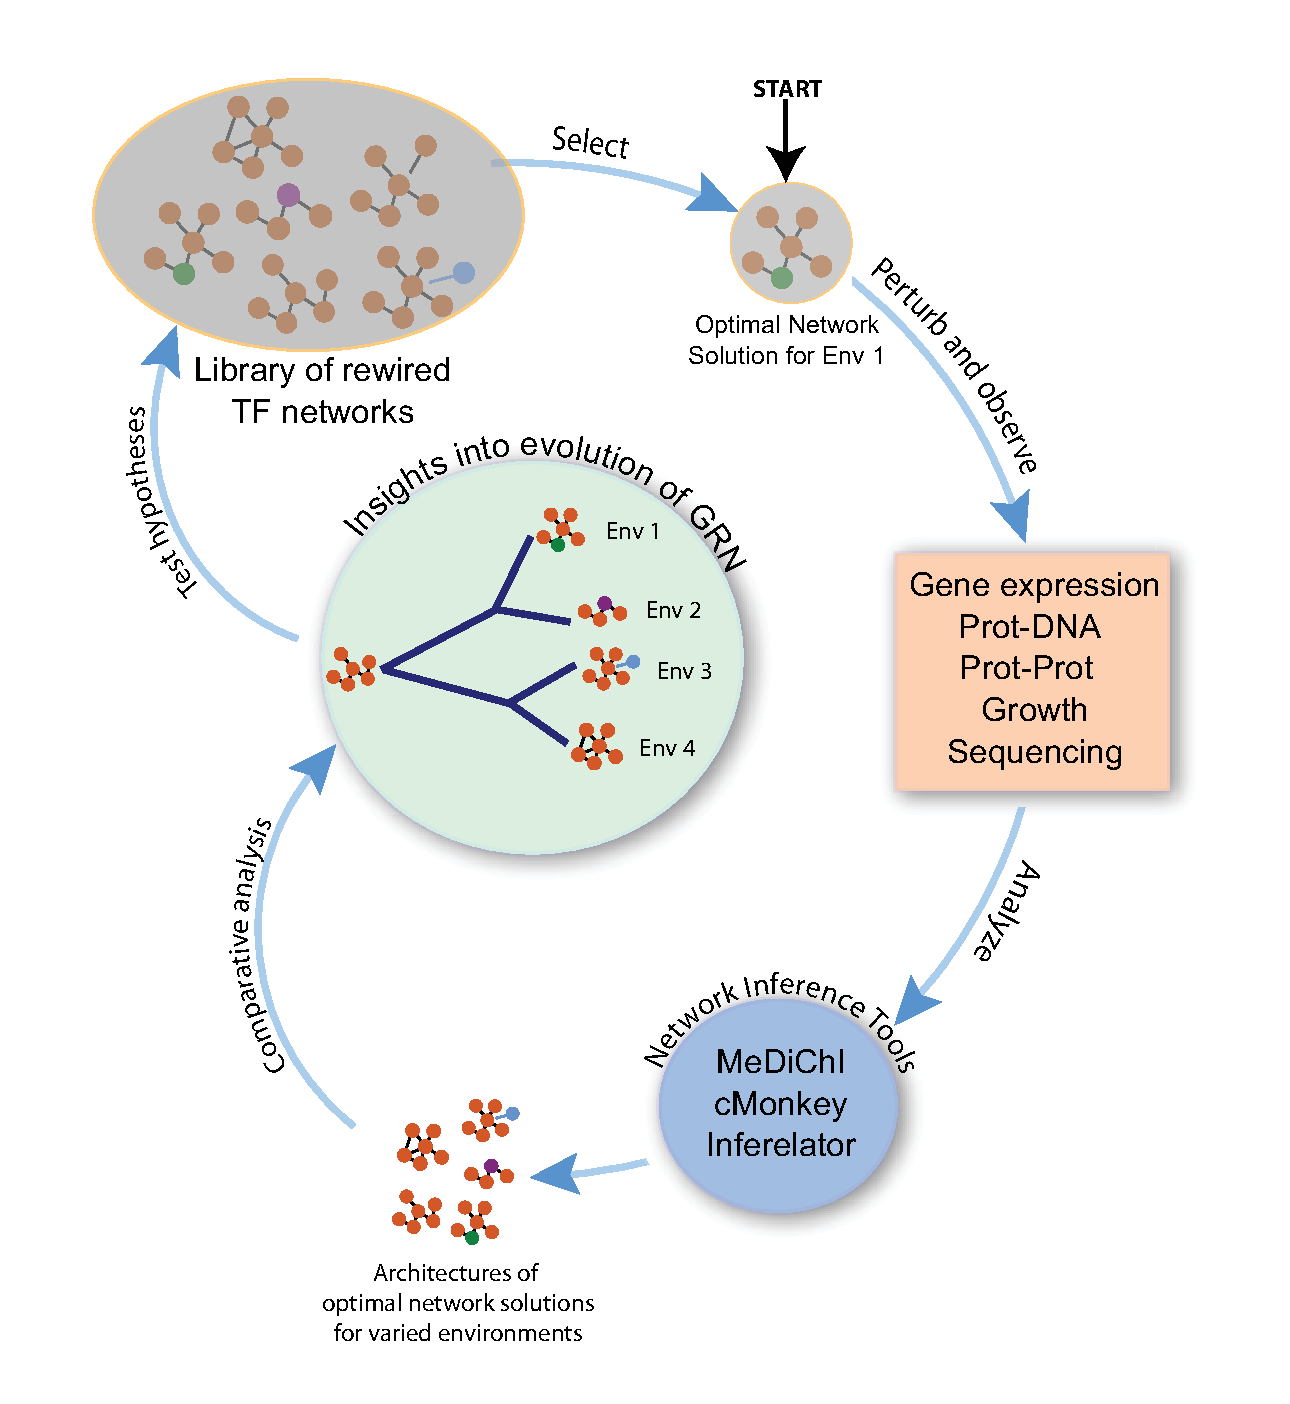
\includegraphics[width=0.65\textwidth]{figures/review_figure3}
 	\caption[Systems approaches to study GRN evolution]{The first step in understanding GRN evolution starts with a naturally evolved GRN that has increased fitness in a given environment. Initially, the architecture of the network is unknown (indicated by gray shading). To delineate the connectivity of the network, we perturb it via genetic or environmental alterations and observe the phenotypic response across multiple data types (orange box). The data is analyzed and integrated using network inference tools to build a comprehensive view of the changes to identify architectures of optimal network solutions (Blue circle). Many iterations of this cycle for different environments yield to library of optimal network solutions which can be compared to derive evolutionary insights (Green circle) and further formulate hypotheses. These hypotheses are tested by construction of rewired GRN by introducing variations at specific components (Gray ellipse). Rewired GRN are selected at different environments and characterized in the next iteration.
}
    \label{fig:chap6:network_inference}
\end{figure}

\subsection{Current limitations}

\subsubsection{Challenges of using comparative genomics alone}

Since the completion of the first bacterial genome-sequencing project in 1995 \cite{fleischmann_whole-genome_1995}, the number of completely sequenced organisms has increased rapidly.  While initial studies confined themselves to a narrow spectrum of phylogenetic diversity, newer sequencing efforts have leveraged known 16s rRNA associations to suggest additional organisms and lineages whose gene sets may be under sampled \cite{wu_identification_2009}. Beyond sequencing the genome of a single species, recent metagenomic studies attempt to capture the genetic diversity present in complex environmental samples, characterizing novel genes from a number of microbial species that are uncultured under standard laboratory conditions \cite{handelsman_metagenomics:_2004,streit_metagenomics_2004}. Whole genome sequences from organisms spanning diverse evolutionary domains have enabled comparative analysis between closely \cite{edwards_co-operative_2002} and distantly related species and lineages \cite{koonin_structure_2002,makarova_hicab_2006}. Orthology between genes in separate lineages can suggest similarity in function \cite{tatusov_cog_2000}, participation in common pathways \cite{kanehisa_kegg:_2000}, and shared regulatory motifs \cite{kellis_sequencing_2003}, although the precise mechanisms behind co-regulation of similar genes is often markedly different between species \cite{wapinski_gene_2010}. A challenge of comparative approaches, however, is to separate adaptive events from exaptive events; that is, to isolate those events that are either random (i.e. the result of genetic drift) or structural consequences of other acquired traits \cite{gould_spandrels_1979}. Exaptations can be prevalent even between closely related species.  For instance, small changes in gene regulatory circuits have resulted in substantial diversification of closely related species.  In the fungi \textit{Kluyveromyces lactis} and \textit{Candida albicans}, the combinatorial circuits regulated by Mcm1 have diverged significantly \cite{tuch_evolution_2008}  through gain or loss of Mcm1 binding sites and combinatorial associations with other transcriptional cofactors. After ~300 million years of divergence between \textit{S. cerevisiae} and these two fungal species, only 15\% of the direct Mcm1-target gene interactions remain intact.  Determining which of the myriad genetic changes results in increased fitness in new environments is a challenge for laboratory experimental evolution studies. In the subsequent sections, we consider experimental methodologies to characterize molecular mechanisms that drive cellular adaptation to new environments. 

\subsection{Experimental challenges and opportunities}

\subsubsection{Laboratory evolution (directed selection)}

Experimental evolution studies have changed our understanding of short-term adaptation in microbial populations.  A common strategy employed in these studies is to enrich, over several generations, mutants that are better suited to propagate in a gradually changing environment.  In such experiments adaptation to new conditions (improved fitness relative to the ancestral genotype) emerges quickly, within a few to hundreds of generations depending on the type and severity of stress.   Perhaps most well-known and celebrated are Richard Lenski's long-term evolution studies in \textit{E. coli}.  In an early study, Travisano and Lenski propagated 12 replicate \textit{E. coli} populations for 2,000 generations in a glucose-limited environment \cite{travisano_long-term_1996}. To assay for increased fitness, the authors competed these evolved strains against their ancestor in 11 novel, single-nutrient environments. In cases where the uptake mechanism of the novel nutrient is similar to glucose, the evolved strains exhibited similar levels of increased fitness; in response to nutrients with uptake mechanisms different than glucose, however, the strains behaved more unpredictably, suggesting that each strain achieved adaptation to glucose limitation by an independent mechanism.  In follow up to this work, Blount et al. reported the adaptation of \textit{E. coli} to growth in minimal glucose supplemented with citrate \cite{blount_historical_2008}. Wild-type \textit{E. coli} cannot utilize citrate as a carbon source under oxic conditions. The adaptive ability of \textit{E. coli} to utilize citrate manifested after 33,127 generations and over twenty years of growth under selective conditions. Adaptation of this novel functionality likely required at least three genetic changes. While the exact location and type of mutations are still unknown, the authors suggest that the adapted \textit{E. coli} strains, which have the ability to metabolize citrate but lack the ability to transport it into the cell, may have activated a cryptic citrate transporter. This study is of particular importance both because it demonstrates the emergence of novel functionality during the course of a laboratory experiment and suggests that mutational events have historical contingency. Without at least two ``potentiating'' mutations in the genetic background, citrate metabolism evolved infrequently. Most recently, Barrick et al. compared the rates of genomic evolution and adaptation in \textit{E. coli}. They confirm the long-standing observation that adaptation slows considerably after several thousand generations \cite{lenski_quantifying_1991} and demonstrate that the rate of genomic mutation remains relatively constant for as many as 20,000 generations \cite{barrick_genome_2009}. Surprisingly, most mutations observed in this experiment were beneficial. Taken as a whole, this body of work illuminates important evolutionary mechanisms and raises important questions regarding the reproducibility of adaptation, duration in the periods of rapid evolution followed by stasis, and the role of chance events like mutation and drift in adaptive evolution. Later on we will discuss how complex genetic interactions also play an important role in defining the constraints of adaptive evolution \cite{lenski_dynamics_1994}.  

Studies in \textit{Pseudomonas fluorescens} SBW25 have also elegantly demonstrated the evolution of novel phenotypes under laboratory conditions \cite{beaumont_experimental_2009}. Depending on conditions of growth (shaken or static), \textit{Psuedomonas} genotypes retain close resemblance to their ancestor or they diversify into a range of sub-types that can occupy unique environmental niches.  Remarkably, when subjected to a fluctuating environment that alternately favors one of two phenotypes, \textit{P. fluorescens} evolves bet-hedging mechanisms that permit stochastic switching between the two phenotypes.  Similar to Lenski's finding, Beaumont \textit{et al.} report a limited number of genotypic differences (nine in this case) between the evolved strain and its ancestor. Surprisingly, the final requisite mutation can be attributed to a single non-synonymous mutation in the large subunit of carbamoylphosphate synthetase (\textit{CarB}), a central enzyme in the pyrimidine and arginine biosynthetic pathways. Similar to Lenski’s finding, the final mutation required an accumulation of previous, potentiating mutations, suggesting that complex epistatic interactions between genotypes drives the evolution of novel phenotypes.  The methodology in this experiment is of particular interest for future experimental evolution studies, as the authors achieve this new phenotype rapidly by imposing bottlenecks on the population structure at each \"selection\" event. 

A consistent conclusion from these laboratory studies is that significant improvements in fitness are gained through simple mutations in few to single genes.  Functional mutations typically reside within the coding region of genes and presumably alter the kinetics or substrate specificity of proteins, although recent studies suggest that simple mutations in some non-coding elements, such as riboswitches, can also confer selective advantage \cite{tremblay_c-type_2011}. Such findings, however, are inconsistent with comparative genomic studies, which suggest that regulatory rewiring of cis-regulatory elements is a primary source of early diversification between species.  Theoretical insights similarly suggest that modularity, which is the result of regulatory programs, is critical for the robustness and adaptability of living systems \cite{kitano_biological_2004}. Many of the adaptive features that allow an organism to robustly respond to changes in its environment are encoded at the level of gene regulation -- how genes are turned on and off, where and when they are expressed, and what controls their expression (forming the modularity observed in living systems). This raises interesting questions regarding failure of laboratory studies to enrich mutants with improved fitness that results from alterations in GRNs. 

One plausible explanation is that the types of selective pressures used in these studies can be generally categorized as simple nutritional stress. If so, selection with repeated patterns of complex, dynamically changing environmental conditions should enrich for regulatory mutants that can reversibly readjust physiology in novel ways.  The study that comes closest to this design is the one conducted by Tagkopolous et al \cite{tagkopoulos_predictive_2008}. In this study the authors enriched a population of \textit{E. coli} with improved fitness to artificially decoupled changes in oxygen and temperature in less than 100 generations. Although the authors did not characterize the mechanistic underpinnings of this improved fitness phenotype, one can speculate that alterations to the GRN structure is the only plausible mechanism to reverse the naturally evolved relationship among processes independently attuned to handle temperature and oxygen-related physiologies. Regardless, we should recollect that selection is a very powerful tool in evolution. While selection imposed by altering a single factor might facilitate analysis and interpretation of adaptive mechanisms discovered in the lab, it does not accurately mirror processes in natural environments, where multiple variables change simultaneously. Environmental heterogeneity and complexity are important and ubiquitous factors in the evolution of natural populations. Interactions among genes, mutations, and environmental factors contribute to adaptability, defining the landscape in which organisms evolve. Heterogeneous environments may create rugged fitness landscapes that contain a multitude of local fitness optima, many of which may be explored by a natural population \cite{cooper_experimental_2010}. Simulations suggest that varying environments can actually speed up the rate of evolution \cite{kashtan_varying_2007}, especially when new environmental goals are modular – sharing features present at early times. Combinatorial and sequential experimental designs, where cells are exposed to varying sequences or combinations of pressures may reveal natural couplings between environmental events that have been learned by cells \cite{baliga_systems_2008} and in long-term studies may suggest how organisms anticipate and respond to complex environmental changes.

It is also important to keep in mind that regulatory rewiring events, though fast on an evolutionary timescale, may still require over thousands to millions of years, far beyond the scope of a typical laboratory experiment.  Approaches that introduce vast amounts of variation into targeted genetic elements of a natural population prior to selection with an appropriate complex perturbation could circumvent this limitation.  Such strategies, while utilized in the past \cite{wang_programming_2009}, have witnessed renewed interest and enthusiasm because it is now possible to generate fully synthetic genes and genomes \cite{gibson_creation_2010} and comprehensively identify and track mutants in large populations using NextGen sequencing technologies \cite{margulies_genome_2005}.  

\subsubsection{Model systems to study adaptation}

Microorganisms are ideal for studying the molecular basis for physiological adaptation because of the ease with which they can be genetically manipulated and cultured under controlled environments.  In addition, they generally have (i) short generation times, (ii) large effective populations, and (iii) small, relatively simple genomes. These properties allow for rapid, high-throughput surveys of genetic fitness landscapes over relatively short timescales.  Microorganisms commonly employed for molecular evolution studies include \textit{E. coli}, \textit{B. subtilis}, and \textit{S. cerevisiae}. All of these organisms are well characterized, with completely sequenced genomes and a wealth of validated functional annotations.  Groundbreaking insights into evolution have been made using each of these organisms. Richard Lenski and colleagues demonstrated adaptation to growth on citrate, where the inability of \textit{E. coli} to proliferate on citrate has traditionally been a characteristic hallmark \cite{blount_historical_2008}. In \textit{B. subtilis}, several groups have studied adaptation in stress response pathways, including sporulation and competence (Reviewed in \cite{hamoen_controlling_2003,errington_regulation_2003}). Finally, the yeast community has produced tremendous work linking gene expression to adaptive evolution \cite{ferea_systematic_1999}.  Halophillic archaea, like \halo, are an especially powerful system in which to study the evolution of cellular stress defense mechanisms as they have evolved in constantly fluctuating and extreme environments, including salinity (10 times that of seawater; 2.5-5.0M), light (>150μmol photons/m-2/s-1), oxygen (<5 μM), temperature (30ºC–50ºC), nutrients and DNA damaging agents such as UV radiation. Like \textit{E. coli} and \textit{B. subtilis}, \textit{H. salinarum} is relatively simple, readily manipulated, and has a smaller completely sequenced genome (~2,400 genes). All of these features make it an appealing system to disentangle the complex adjustments cells undergo in response to variable environmental conditions. In addition, archaea are evolutionarily unique relative to both bacteria and eukarya.  Their basal transcriptional and replication machinery, for instance, shares common ancestry with the eukaryotic machinery, whereas their regulatory systems have bacterial character and they retain the capacity for HGT \cite{baliga_is_2000,geiduschek_archaeal_2005,edgell_archaea_1997}.  Studies in \textit{H. salinarum} are revealing mechanisms by which a GRN acquires complexity through duplication of transcription factors.  By expansion of two eukaryotic general transcription factor families (six TBPs and seven TFBs, TFIIB orthologs) and subsequent changes to the promoters and coding sequences \textit{H. salinarum} has evolved regulatory programs to modulate the expression of large fractions of genes that allow it to rapidly acclimate to changing environmental conditions \cite{whitehead_diurnally_2009,facciotti_general_2007,schmid_single_2009}. 

\subsubsection{New experimental approaches to study GRN adaptation} 

We are witnessing unprecedented advances in technologies for probing biological phenomena.  Powerful high-resolution and high-throughput experimental and computational tools are being used to tackle old biological questions and discover new, often-unanticipated avenues for research. These tools have changed ways in which we think about biological systems, generate hypotheses, and execute experiments.  When the first complete genome of a microorganism was sequenced fifteen years ago \cite{fleischmann_whole-genome_1995}, sequencing a several megabase genome in a day was unimaginable. Now, NextGen sequencing technologies continually push the limits of quality, quantity and cost of sequencing runs. As the cost of these technologies decreases, they are becoming more widespread.  Together, these tools give investigators unprecedented access to the signatures of evolution; by comparing larger numbers of related and diverse genomes, and as they occur within laboratory experiments.  For instance, we can observe within the time frame of a laboratory experiment evolutionary processes that normally occur over thousands to millions of years in natural environments.  We can do this by accelerating evolution using automated multiplexed culturing devices to enrich mutants from microbial populations containing large numbers of random or semi-random variation generated using a combination of gene synthesis and mutagenesis technologies. By using NextGen sequencing, whole genome oligonucleotide arrays, metabolic arrays and mass spectrometry, and high-throughput protein quantitation, it will be possible to link phenotypic outcomes to genetic changes and characterize adaptive mechanisms responsible for improved fitness in new environments. Such forward-looking approaches are exemplified by an experiment in which Wang et al identified one mutant with fivefold increased lycopene production within 3 days from a population of 4.3 billion \textit{E. coli}  \cite{wang_programming_2009}. The key technologies used in this remarkable proof-of-concept study included multiplexed automated genome engineering (MAGE) to introduce combinatorial variation into the \textit{E. coli} EcHW2 genome and clever bottlenecking and selection approaches.  The combination of these technologies accelerated the emergence of multistep phenotypic adaptations that may have otherwise been extremely improbable due to transient decreases in fitness or genetic drift \cite{beaumont_experimental_2009}.  Especially with respect to GRN evolution, the ability to generate vast amounts of genetic diversity rapidly, followed by deep sequencing of mutants with increased fitness will give us a lens into long-term evolutionary processes that would otherwise be inaccessible.  Finally, synthetic approaches that directly manipulate pre-existing cellular architecture can rapidly accelerate evolutionary processes and confirm or repudiate hypothesis of adaptive mechanisms suggested by laboratory evolution or comparative genomics studies. Directly manipulating gene regulatory networks is a powerful approach to disentangle complicated evolutionary scenarios discovered by comparative approaches.  Isalan \textit{et al}, for example, studied the effects of regulatory circuit rewiring in \textit{E. coli} by swapping \textit{cis}-regulatory and downstream DNA binding domains of TF genes across the TF hierarchy \cite{isalan_evolvability_2008}.  They observed that most rewiring events are neutral under standard growth conditions and can even be advantageous under some stress conditions. Although the phenotypes monitored in this experiment may not fully reveal the consequences of GRN rewiring, the authors suggest that higher-order control of GRNs may minimize the impact of transcriptional rewiring and that such cost-free tinkering with gene regulatory circuits may be a common mechanism in the evolution of GRN.  It will be interesting to assess how often this is the case in more complex environments, where the effects of misregulation may manifest themselves more dramatically and to validate the molecular phenotypes of GRN rewiring by gene expression profiling. 

\subsubsection{Evolution of microbial communities} 

Part of the complexity of natural environments is a product of interspecies dynamics. Members of ecological communities influence each other by altering their natural environment, competing for common resources, cooperating with one another to solve common challenges, complementing each other’s nutritional needs and preying on one another.  Interspecies interactions directly influence natural selection by modifying the selective criteria imposed by the environment.  The evolution of a single species is tightly coupled to the co-inhabitants of its environment. Importantly, the evolution of a species in isolation may proceed differently when that same species evolves in the presence of other organisms. Competition between \textit{S. pneumoniae} and \textit{H. infuenzae} for colonization of mucosal surfaces, for example, drives S. pneumoniae to develop opsonophagocytosis-resistance, which is associated with invasive nasopharynx diseases. In the absence of \textit{H. influenzae}, this resistance mutation bears a fitness cost; yet, in competition with \textit{H. influenzae}, which actively stimulates neutrophil-mediated opsonophagocytosis, the resistance mutation becomes advantageous \cite{lysenko_within-host_2010}. Besides adjusting to varied selective criteria that are the consequence of interspecies dynamics, cells in natural environments have access to vast pools of genetic material with which they can diversify and innovate. The prevalence of horizontal genetic diversity within microbial populations was severely underestimated until recently (Reviewed in \cite{koonin_horizontal_2001}). Faced with stressful conditions that are difficult to address with existing molecular parts, an organism may look outward to find genes that increase its likelihood of survival.  Many microorganisms maintain conserved pathways through which they become competent to uptake DNA from the environment.  In \textit{B. subtilis}, the activation of competence is mediated by noise in expression of the regulator ComK \cite{schultz_deciding_2009,maamar_noise_2007}. Given stressful conditions, \textit{B. subtilis} dedicates approximately ten percent of its population to survey the environment for new survival strategies. Such mechanisms can dramatically increase the rate of evolution in asexual populations.  Another important property of microbes that has only recently been appreciated is genomic plasticity, which refers to variation in genome architectures across individuals of a natural population.  It is becoming increasingly evident that microbial populations are rife with genomic variability, bringing into question the definition of a microbial species itself \cite{smith_how_1993,achtman_microbial_2008}. Together, genomic plasticity and metabolic flexibility (the ability of organisms to reversibly adjust biochemical capability by regulating gene expression and enzyme activities) increases the adaptive capability of a microbial community.   

\subsubsection{Insights into mechanisms of adaption and future directions} 

We have reviewed known mechanisms by which organisms adapt to new environments and made a case for integrating computational and experimental approaches to study this process and discover new mechanisms. It should be noted that while new technologies have increased the resolution and scale at which we can probe evolutionary processes, they do not override the need for well-designed experiments. Carefully designed selection pressures and culturing technologies will decide the degree to which adaptive mechanisms uncovered in laboratory studies accurately reflect natural processes. The ultimate test of our understanding of how cells adapt will come from surveying variations within related populations that have evolved naturally to deal with varying environments. This is feasible to do as we now have the capability to determine complete metagenome sequences using sequencing technologies. It is important that we iteratively refine our models so findings from the laboratory are brought into close apposition with what we are able to observe in a natural environment. Knowing the mechanisms by which organisms evolve will eventually equip us with better engineering principles and strategies to synthetically alter their capabilities. Such rational reengineering has very important implications for how we can address environmental and health related problems in the future \cite{koide_role_2009}.  

\subsubsection{Intelligence in Microorganisms}

An intriguing question emerging from experimental evolution studies and studies of regulatory networks in microbes is whether microorganisms are capable of ``intelligence''. For centuries, mankind has grappled with the precise nature and defining features of intelligence. Debates have erupted over how to define and measure the extent of intelligence in parts of the biological (and non-biological) world. Alan Turing, for example, famously proposed a test for evaluating the performance of ``artificial intelligence'': namely, can it be distinguished from the performance of human beings by another human \cite{turing_computing_1950}? There have also long been philosophical discussions on what can be considered intelligent. A number of studies have explored whether there are differences in intelligence between human populations \cite{neisser_intelligence:_1996}, whether animals \cite{thorndike_animal_1998} and even plants \cite{trewavas_mindless_2002} exhibit intelligent behaviors, whether non-human artificial systems are capable of intelligence \cite{brooks_intelligence_1991} and, more recently, whether intelligence spans biological domains including even the simplest of microbes \cite{hellingwerf_signal_1995,bruggeman_macromolecular_2000,hoffer_autoamplification_2001,ben_jacob_bacterial_2004}. 

As an abstract concept, intelligence escapes easy definition. As a linguistic construct, its characteristics have varied substantially across philosophical and cultural contexts. Rather than launch an ontological, epistemological, or semantic inquiry, I ask instead whether there is scientific utility in assigning intelligence to microbes? Is it possible that mathematical perspectives of complex adaptive systems and recent data-intensive developments in systems biology will help us detect and define microbial intelligence? Would viewing microbes through the lens of intelligence can help us better describe their behavior, harness their intelligence to perform valuable actions and, in the end, possibly extend our understanding of the human brain itself?

The modern biological perspective of intelligence, even at its most fundamental level, tends to associate it with the human brain. In this context, intelligence is a property of the human brain, or a feature that somehow emerges from its activity. Accepting that intelligence may not be exclusively a feature of the human brain, but rather it may be present – at least to a degree – in all creatures possessing brains or nervous systems, already helps refine the general features of intelligence. However, intelligence may not have to be associated solely with a certain biological organ, such as a brain or a nervous system. Brains and nervous systems may be highly adapted conduits for expressing and integrating multiple intelligent behaviors. Some of these behaviors may be exhibited by other complex adaptive systems present in living organisms that do not have a brain or nervous system. As early as 1995, Hellingwerf suggested that some two-component systems in bacteria comply with the requirements for elements of a neural network \cite{hellingwerf_signal_1995}. More recently, the so-called biogenic approach of cognition has gained momentum by focusing on the biological origin of cognition and intelligence, abandoning a strict anthropocentric perspective \cite{lengeler_metabolic_2000,lyon_biogenic_2006}.

A recently submitted manuscript provided in Appendix \ref{appendix:a} provides examples of intelligence in the microbial world. It argues that, at least for some specific tasks, microbial intelligence can be compared to human intelligence, i.e., microbial networks can be considered formally ``intelligent''. Recognizing microbial intelligence may allow us to modify microbial networks or develop new microbial networks capable of intelligent solutions to specific human problems \textit{de novo}. Alternatively, if intelligence (or components thereof) emerges from the dynamics of complex adaptive systems and the human brain is an evolved organ for the encapsulation of intelligent characteristics, then it is possible that there may be features of intelligence that remain undiscovered.

\section{Inference, visualization, and dissemination of GRNs} 

The above section described several directions for experimental studies that accurately reflect evolution in natural environments, or introduce changes into organisms that accelerate the process of evolution itself. To leverage the power of these new biological insights, we must integrate data into intuitive-yet-accurate models within which investigators can interactively explore functional relationships among genes and generate new hypotheses. As system-wide data becomes more available, it is increasingly important to develop computational methods to handle diverse data types, both individually and collectively. Important advances in the area of network inference have been made over the past several decades. From high-resolution kinetic models to abstract Boolean representations, the field of network inference is rapidly growing in sophistication. 

\subsection{Challenges and opportunities: GRN inference}

Numerous advances have been made in GRN inference, including what has been described previously in this manuscript.  In the past, studying the function or evolution of GRNs presented a formidable challenge, even for model organisms with relatively small genomes.  It took considerable effort to develop molecular and computational tools to map all regulatory connections to construct reliable network models.  Even in this regard ``well-defined'' GRNs were sparse and mostly restricted to a select few model organisms including \textit{E. coli} \cite{salgado_regulondb_2006,madan_babu_evolution_2003}, yeast \cite{lee_transcriptional_2002} and \textit{B. subtilis} \cite{moreno-campuzano_identification_2006,makita_dbtbs:_2004}.  Despite the obvious limitations that come with poor taxonomic coverage of such model organisms, comparative analysis of their GRNs did identify three major mechanisms driving GRN evolution (see Figure \ref{fig:chap4:evoGRN}): (i) alterations in TF-target gene interactions, (ii) gene duplication followed by subfunctionalization or neofunctionalization, and (iii) horizontal gene transfer events  between species.  Since there were few experimentally derived models of GRNs, investigations relied on \textit{in silico} models whose components include synthetic genes that evolve according to rules encoded in a computer simulation \cite{wagner_genetic_1996,milo_superfamilies_2004,siegal_functional_2007}.  Although \textit{in silico} approaches are extremely informative and will continue to yield valuable insights, they grossly underestimate complexity of naturally evolved GRNs \cite{de_smet_advantages_2010}.  There are now increasingly sophisticated methods for inferring the structure of GRNs from high-throughput systems biology data \cite{bonneau_learning_2008,gardner_inferring_2003}, (Figure \ref{fig:chap6:network_inference})  

It is important to recognize that key to the success of these inference procedures is the quality, quantity and types of data.  Well thought out experiment designs are critical to build models that are predictive and mechanistically accurate.  These experiments should appreciate the fundamental properties of biological processes in that they are dynamic, probabilistic and conditional. Through application of these approaches there is now an ever-increasing number of experimentally verified GRNs \cite{de_smet_advantages_2010}. Such systems level investigation has and will continue to revolutionize how we investigate and understand cellular adaptation to a new environment through the evolution of complex GRNs.

High-throughput methodologies generate a wealth of data. Consolidating diverse data types into coherent models of biological interactions and their functional consequences will be critical for understanding systems-level adaptive processes. This presents a challenge for traditional computational tools, which generally represent biological networks as static, uni-dimensional entities. Evolutionary systems biologists, however, are interested in how the structure of multi-dimensional biological networks changes as a result of adaptation and how these alterations in network properties affect dynamic cellular processes and their associated downstream phenotypes. While systems approaches have been successfully applied to a number of biological problems, including abstract boolean network analysis of cell-cycle attractor states \cite{li_yeast_2004}, flux-balance models of metabolism (Reviewed in \cite{kauffman_advances_2003}), and causal biclustering methods for transcriptional regulation \cite{bonneau_predictive_2007}, to elucidate evolutionary mechanisms future models must (1) integrate across diverse biological processes, (2) represent biological information across multiple time scales with varying degrees of resolution, and (3) develop network representations that track changes in network structures over long (evolutionary) timescales. Such advances will be made by harnessing interdisciplinary approaches, leveraging insights and expertise from a number of disciplines, including mathematics, computation, physics, and engineering. The workflow by which systems-methodologies can be applied to experimental evolution studies is depicted in Figure \ref{fig:chap6:network_inference}.

In parallel, advances have been made in statistical machine learning, including the ensemble learning frameworks described in Chapter \ref{chap:2}. As the number and diversity of data types increases, there will be opportunities to integrate multiple algorithms that each learn from a single data type into an ensemble. This way multiple aspects of biology can be captured in a single model. The primary challenge will be to build analytical frameworks that accommodate fundamentally different types of predictions and associations (e.g., \textit{cis}-regulatory motifs, co-regulation, protein-protein interaction, kinetic, etc. in a single model). These future models will also have to weigh the level of detail at which they intend to model the biology. Most important, these models should be constructed to address specific biological questions. Finding that appropriate level of abstraction will depend on the problem - there will not be one-size-fits-all solutions.  

\subsection{Challenges and opportunities: GRN visualization and dissemination}

Having inferred models from data, a next step is to make that information useful to investigators. This is especially important given the increasing size and complexity of these models. A single \egrine model, for example, consists of hundreds of thousands of biclusters and motifs, not to mention accessory functions and additional data. The footprint of each model is on the order of tens of gigabytes of hard drive space and loading the ensemble requires a file-backed memory management system because the models are too large to fit into active memory on current machines (e.g., $>$8GB). That's not even to mention the computational time and power to construct the model in the first place. To facilitate exploration of the model's predictions by biologists and other researchers in our group, I designed a comprehensive web-framework. All of the model predictions are hosted in a PostgreSQL database that is queried by a web application framework called Django. Django uses a model-view-controller (MVC) framework to dynamically generate content for users requesting a specific page. It consists of (1) an object-relational mapper that manages data models (i.e., Python classes) and a relational database (the ``Model''), (2) a web templating system for generating viewable content from the models (the ``View'') and (3) a regular-expression-based URL dispatcher (the ``Controller''). In addition to the base Django functionalities, we also developed a genome browser, $iGB^{web}$, to emphasize model dynamics. For every gene in the model, the user can examine the relative influence of each GRE on co-regualtion of the gene in context of each corem to which it belongs (see Figure \ref{fig:corem_gres}). A paper describing $iGB^{web}$ is provided in Appendix \ref{appendix:b}. The \egrine\ website is available at: \href{http://egrin2.systemsbiology.net}{http://egrin2.systemsbiology.net}

Encoding biological information in a graphical representation has proved valuable for analyzing GRNs and discovering critical topological determinants of information flow in other contexts as well. Models of GRNs can be made accessible through visualization software with user-friendly interfaces, such as Cytoscape \cite{shannon_cytoscape:_2003}, BioTapestry \cite{longabaugh_computational_2005}, and Gephi \cite{bastian_gephi:_2009}.  By interoperating with other software and databases on the desktop or via the internet using frameworks such as Gaggle \cite{shannon_gaggle:_2006} and Firegoose \cite{bare_firegoose:_2007}, scientists can explore the complex networks and disparate data types to formulate hypotheses and drive experimentation. Application of these frameworks is turning increasingly to the web. Several projects like BioJS \cite{gomez_biojs:_2013} - a modular JavaScript library for reusable interfaces - have attempted to increase biologist's ability to interact with their data on the web.

\section{Towards a dynamical interpretation of genetic co-regulation: what do corems mean?}

Corems expand the lexicon of genetic regulation. They make us reconsider what we mean by the term ``co-regulation''. Would, for example, a map of the direct interactions between every TF and every gene be sufficient to understand expression of the genome? From a dogmatic position centered around operons and regulons, it should. If genes are regulated by a common factor, they should be co-expressed. One might have to account for some combinatorial interactions that alter expression (Figure \ref{fig:chap5:combinatorial_reg}), but at least in microbes combinatorial interactions are somewhat rare. We would also expect from this perspective that genes with common functions will be physically bound by the same factor. While this is certainly the case for many genes and functions, this limited perspective misses an entire side to co-regulation that has an enormous impact on cellular fitness. Corems can model these relationships.   

\begin{figure}[h!]
    \centering
    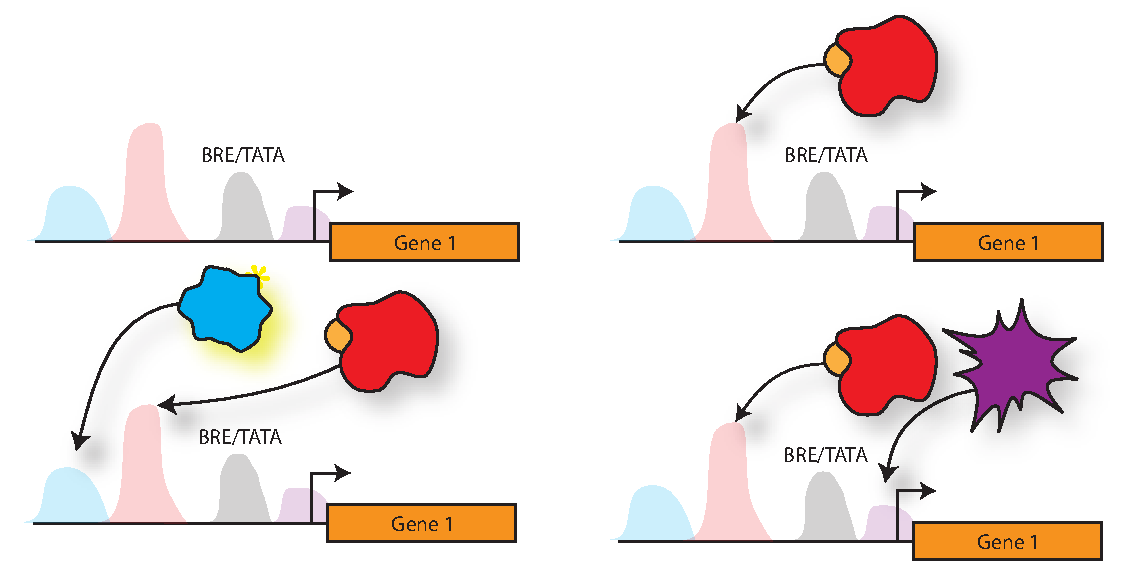
\includegraphics[width=0.9\textwidth]{figures/combinatorial_reg}
 	\caption[Combinatorial regulation at gene promoters shapes gene expression]{Multiple TFs can bind to a gene promoter. Binding of multiple TFs can be synergistic to promote transcription (bottom-left) or cause interference that reduces expression (bottom-right). 
 	}
\label{fig:chap5:combinatorial_reg}
\end{figure}

What has been missed in these definitions is the role of dynamics in transcriptional regulation - both at the level of physical interactions between TFs and DNA at gene promoters, and the dynamical properties that influence TF activity, like allosteric binding to small molecules. Most studies have emphasized strictly defined physical binding of common TFs to be ``co-regulation''. I have two concerns with this definition: (1) not all genes bound by a common TF are co-expressed. This is very clear from gene expression data. Many members of regulons are not highly co-expressed. At the moment, this cannot be accounted for by combinatorial influences. This means that it is difficult (if not impossible) to predict whether two genes will be co-expressed knowing that they are bound by a common TF. (2) Genes bound by different TFs can be co-expressed across many environments (more tightly than genes bound by a common TF). This is one of the observations that motivated formalization of corems. It turns out that oftentimes these genes (even though they have no evidence for common direct transcriptional regulation) also have highly similar impact on fitness (functioning in related pathways). This suggest that there are transcriptional programs beyond direct regulation that contribute to the emergence of genetic expression modules. Two mechanisms for this behavior are proposed in Figure \ref{fig:chap5:equif} and Figure \ref{fig:chap5:iso}.

\begin{figure}[h!]
    \centering
    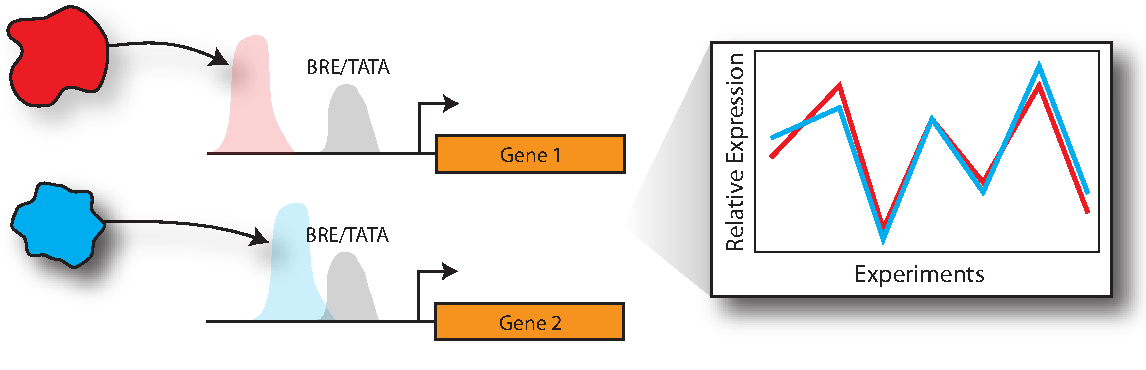
\includegraphics[width=0.9\textwidth]{figures/equif_iso}
 	\caption[Co-regulation beyond common TF interaction]{Despite being physically bound by different, genes can nevertheless be tightly co-expressed across a broad range of environmental conditions. Oftentimes we have also discovered that genes regulated in this way have similar impacts on fitness, suggesting they play conserved functional roles. Is it possible that there are higher-order mechanisms responsible for coordinating their co-regulation?}

\label{fig:chap5:equif_iso}
\end{figure}

\begin{figure}[h!]
    \centering
    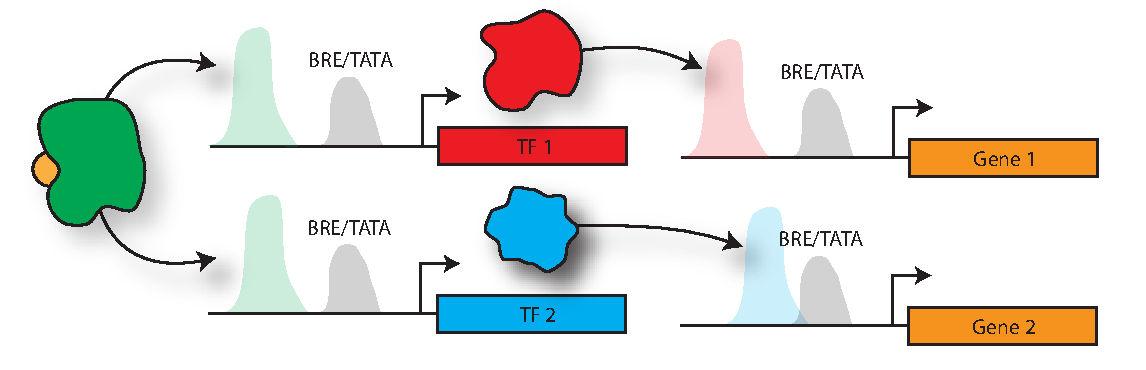
\includegraphics[width=0.9\textwidth]{figures/iso}
 	\caption[Indirect co-regulation by isomorphy]{One conceivable way two genes with distinct direct inputs could produce similar expression is if the TFs themselves were coordinated by a similar factor (i.e., the TFs are isomorphic). This is likely to occur in biological networks and is identifiable directly from GRN topology. 
 	}
 \label{fig:chap5:iso}
\end{figure}

\begin{figure}[h!]
    \centering
    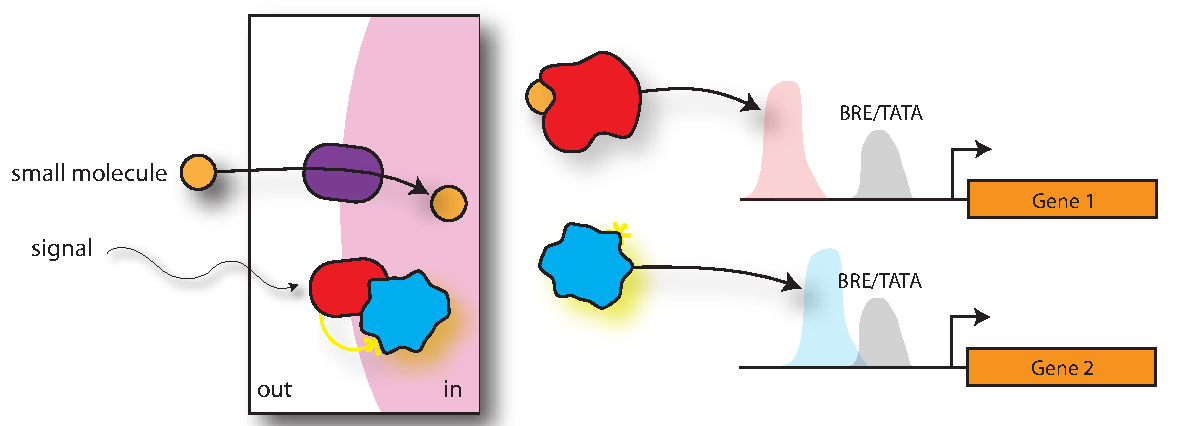
\includegraphics[width=0.9\textwidth]{figures/equif}
 	\caption[Indirect co-regulation by equifinality]{A more complicated way two genes with distinct direct inputs could be co-expressed is through allosteric coordination of TFs. TF activity is often regulated post-translationally. In prokaryotes, this is often by binding to small molecules, called allosteric regulators. If these small molecules cause TF activities to be similar (especially if the two small molecules were related by chemical transformations such that they often change together), the genes regulated by those TFs could exhibit similar expression patterns.   
 	}
\label{fig:chap5:equif}
\end{figure}

While it remains to be demonstrated directly whether these observations have a mechanistic basis, it suggests that coherent expression and coordination of the genome is a system-level property. There are many factors beyond transcription initiation to consider. With a fully detailed model of the cell (all parameters, rates, mechanisms, etc.), prediction of cellular expression state may be possible from GRN topology. Until that time, our results suggest that we take a more phenomenological view of co-regulation - focusing instead on the ``emergent'' modular states that are defined by (sometimes indirect) co-regulation. 

\section{Beyond the GRN}

In Chapter \ref{chap:1} I referred to an article by Neidhardt and Savageau entitled, ``Regulation Beyond the Operon''. It was clear even from the earliest investigations that regulation of the genome was more complicated than co-linear arrangement of genes. I suggest that we also move beyond gene regulation - beyond the GRN. What this thesis work suggests is that genetic regulation involves the entire biochemical milieu of the cell, especially metabolite and protein dynamics. At the moment, we can generate insight by modeling ``emergent'' features of the system (like corems) - with limited understanding of how these features are generated. Future work needs to explicitly model and integrate these layers. This is becoming possible with technological advances in metabolomics and proteomics. Like sequencing of the genome, generation of a completely accurate GRNs may produce more questions than it would answer.  




 

 
 